\documentclass{kththesis}

\usepackage{csquotes} % Recommended by biblatex
\usepackage{biblatex}
\addbibresource{bibliography.bib} % The file containing our references, in BibTeX format

\usepackage{graphicx}
\usepackage{listings}

\title{Providing Software Diversity by LLVM MIR Transformation using Unison}
\alttitle{Varierad Mjukvara genom LLVM MIR Transformation med Unison}
\author{Patrik Karlström}
\email{pkarlstr@kth.se}
\supervisor{Benoit Baudry}
\examiner{Christian Schulte}
\programme{Master in Computer Science}
\school{School of Computer Science and Communication}
\date{\today}


\begin{document}

% Frontmatter includes the titlepage, abstracts and table-of-contents
\frontmatter

\titlepage

% English abstract
\begin{abstract}
	Unison is a tool that combines instruction scheduling and register allocation as a
	single combinatorial problem and solves it using constraint programming, which is a
	programming paradigm for systematically solving combinatorial problems.

	Automated software diversity is the process of automatically providing diverse executables
	in an effort to break so called \textit{gadgets}, which are short instruction sequences
	that together make up an attack vector. Attacks that utilize gadgets rely heavily on the
	arrangement of the code in the executable. By providing a population of executables with
	equivalent functionality but different arrangements an adversary must construct a unique
	payload for each executable. The idea is to mount a proactive defense against
	adversaries and limit the reusability of each constructed payload.

	The results when using Unison to systematically generate diverse executables show that
	the number of possible pairwise distinct executables is often larger than 1000000, even
	for small functions (less than ten instructions). Using Unison to force the executables
	to differ in a particular way is simple to implement, only a handful lines of code. One
	strategy evaluated in the experiment resulted in that the most frequent gadget only
	appeared in 24\% of versions, and 82\% of the gadgets only appeared in one program
	version each.  However, future work is required before anything consumer oriented can be
	evaluated, in part because Unison does not support the x86 architecture.
\end{abstract}


% Swedish abstract
\begin{otherlanguage}{swedish}
  \begin{abstract}
    Träutensilierna i ett tryckeri äro ingalunda en oviktig faktor,
    för trevnadens, ordningens och ekonomiens upprätthållande, och
    dock är det icke sällan som sorgliga erfarenheter göras på grund
    af det oförstånd med hvilket kaster, formbräden och regaler
    tillverkas och försäljas Kaster som äro dåligt hopkomna och af
    otillräckligt.
  \end{abstract}
\end{otherlanguage}



\tableofcontents


% Mainmatter is where the actual contents of the thesis goes
\mainmatter

% Introduction
\chapter{Introduction}

The field of \textit{software diversity} is concerned with researching the
causes and effects of diversity in software and software engineering, both in the result
and the process. As an example consider web browsers; There are many different implementations
of what is essentially the same functionality. In the context of security vulnerabilities
of one browser does not necessarily carry over to another \cite{survey}.

One of the applications of software diversity is as a defense to code re-use attacks \cite{survey}.
Code-reuse attacks refers to attacks that diverts program control flow to re-use already
present code in an unintended manner \cite{code-re-use}. For example if an adversary gains
access to a process' stack the address to jump to after a return instruction can be
overwritten and the adversary can choose which instruction to jump to. \textcite{rop}
extended this concept and introduced what is called \textit{return oriented programming}.
Return oriented programming is a code re-use technique were the program control flow is
diverted to a chain of short instruction sequences, dubbed a \textit{gadget}. By carefully
choosing these gadgets an adversary can achieve arbitrary code execution.

However, the adversary relies on the fact that the chosen instruction sequences are always
equivalent across all binary files. I.e an equivalent sequence of instructions is located
at the exact same offset. If, for example, everyone would run their own, structurally
different but functionally equivalent version of the Firefox web browser an adversary would
have to disassemble all variations and construct a unique payload for every target. Thus,
techniques that provide diversity between executables and/or runtimes have been researched
as a defense to these code re-use attacks \cite{survey}.

To understand how two executables can be structurally different but functionally equal
consider an example pertaining the instruction schedule. Say there are two independent
instructions, one of which is part of a gadget. By swapping the place of these two
instructions the gadget is now different, but since the instructions are independent
program functionality is the same. There are many decisions taken by the compiler that are
not necessarily the only valid decision, and if one could explore all combinations of
decisions one could systematically generate the entire population of diversely arranged
but functionally equivalent executables.

Constraint programming is a paradigm for solving combinatorial search problems wherein
the relationship between variables are expressed as \textit{constraints}. It solves problems
such as scheduling, vehicle routing and, in our case, compiling
 \cite{handbook-constraint-programming, unison-docs}. For example, consider the problem
of scheduling working shifts in a store. The variables could be the start and end time
of a shift for one person, and the constraint could be that there are always two employees
present in the store and no one works for more than 8 consecutive hours.

A \textit{constraint solver} takes a problem such as the example above and finds a value
for all the variables such that all constraints are satisfied, or in the case when no
mapping that satisfies all constraints exists proves that such is the case
 \cite{handbook-constraint-programming}. The process of finding these values consists of
\textit{searching} the combinatorial space and either implicitly or explicitly discarding
combinations that cannot be solutions, i.e does not satisfy the constraints.

\textit{Unison} is a tool that uses a constraint solver to schedule instructions and allocate
registers as a single, integrated problem. It operates as a part of the LLVM backend, and
is thus not a standalone compiler. Unison is potentially optimal in the sense that given
enough time, it can generate the optimal instruction schedule and register allocation.
It finds this solution by searching the combinatorial space in a continuous pursuit for a
solution that is better than the last \cite{unison-docs}.

\section{Problem Statement}

It might feel intuitive to provide software diversity by somehow randomizing a part of an
executable, and in fact many have \cite{survey,librando,binary-stirring}, but this
approach comes with a three key challenges; It is difficult to make guarantees about the
resulting population, proving the correctness of the code transformations is challenging
and there is no fine-grained control of the process.

When generating the executables with a random element in the process you cannot make any
guarantees regarding the resulting population. If you generate two executable you cannot
with certainty tell that they are in fact sufficiently different without verifying it. The
risk of them being equal is most likely very small for just two versions, but what if
10000 different version are generated? Or 1000000? At some point the pigeonhole principle
comes into effect, in which case case it would be better to re-use the already generated
code.

By instead systematically generating different variations those sort of guarantees can be
made. If two equal executables are never generated it follows that they are all pairwise
distinct. It also follows that if the code generator is run to termination, all pairwise
distinct versions are generated. There is also opportunity to define exactly what pairwise
distinct entails. The nature of constraint solving lends itself well to this application.
This is where Unison comes in; In addition to its main purpose Unison has potential for
software diversity purposes.

This thesis aims to be an early exploration of a systematic approach to automated software
diversity using a constraint solver, specifically the Unison tool. It aims to evaluate
both the code generator and the generated code. This leads us to the hypothesis that

\say{Systematically generating diverse executables using a constraint solver is at least
as good as basing the diversification process on randomization.}

\section{Motivation}

As mentioned, it is difficult to prove the correctness of code transformations. Perhaps
the most compelling reason to use a constraint solver for software diversity is that for
a combination to be considered a solution, \textit{all} constraints must be satisfied.
Regardless of what unorthodox approach we want to try out we do not need to consider it's
effect on program functionality, since the constraints that ensure a valid program is
generated must still be satisfied. This property makes implementing new techniques
relatively simple. Modifying code while retaining functionality is no easy task, and this
simplifies it greatly.

With the systematic approach there is full control of what changes between versions, and
how much it changes between versions. Instead of introducing randomness into some part of
the compilation process and more or less hope it generates diverse code with low overhead
the systematic approach offers the possibility of properly reasoning about the process and
steering it specific manners. It also yields a greater control of the quality of the
generated code. Limits can be dynamically set in place so that it does not exceed e.g a
certain number of instructions.

\section{Methodology}

This project is an early exploration of the potential benefits of using a constraint solver
for automated software diversity. Specifically, the research will be carried out by
modifying the Unison tool to support generating multiple outputs. Exactly how these
outputs should differ to generate the most diverse population is outside the scope of this
project. With that said, for the purposes of this thesis the modification of Unison will
include three different options of how the resulting code should differ. Both the modified
code generator as well as the resulting population of each invocation of the code generator
will be evaluated. This lends itself well to an experimental approach.

The purpose of the experiment is to evaluate both the code generator and the resulting
code. The evaluation of the code generator will be performed on both quantifiable and
non-quantifiable metrics (such as ease of implementation). The resulting code, which will
be a population of functionally equivalent but differently arranged code, will be evaluated
in a purely quantifiable way.

\section{Ethics and Sustainability}

\section{Overview}


% Background
\chapter{Background}

This section will be about constraint programming, software diversity, LLVM and Unison

% Software diversity section
\section{Software Diversity}

Software diversity is a diverse field, and there is research focusing on different areas
with different goals in mind. However, what they all have in common is the that they are
exploring the potential benefits of engineering diversity within software development.
When talking about software diversity there are a few different classifications and goals
\cite[Section~1]{survey} which will be covered here.

Software diversity has a diverse (heh) set of goals ranging from fault-tolerance to re-usability
to security \cite{survey}.

\subsection{Managed Software diversity}

Managed software diversity is the notion of encouraging or controlling software diversity.

\subsubsection{Natural Diversity}

A lot of software with similar features naturally and spontaneously emerges from engineering
processes. There are a multitude of products from competing organizations that provide
the same function, for example routers, web browsers, compilers, database management systems
and firewalls. Natural diversity could also be something as simple as one program being
tunable by parameters to provide different functionality and performance \cite{survey}.

\subsubsection{Design Diversity}

Design diversity is the process of introducing diversity through the design process. For
example, \textit{N-version programming} is the approach where $N \geq 2$ functionality equivalent
programs are developed from the same specification. The point of this is that hopefully
it will result in a subset of the programs being free from bugs that another subset
might suffer from, thus creating a more fault tolerant system \cite{n-version}.

\subsection{Automated Software Diversity}

\textcite{survey} describes automated software diversity as \say{techniques for artificially
and automatically synthesizing diversity in software} \cite[\pno~8]{survey}. It is also
known as \textit{synthetic diversity} \cite{synthetic-diversity}. \say{Automated} is
referring to the fact that a human is not part of the diversification process, other than
having designed the framework \cite[Section~4]{survey}.

Automated diversity can characterize itself in different ways. A common approach is to
introduce some kind of randomness into software to break the otherwise deterministic behaviour
of most software. This can have several benefits, including security \cite{add-obfuscation}.
Randomization techniques are generally ways to either directly or indirectly create unique
execution of the same program \cite[Section~4.1]{survey}.

\subsubsection{Dynamic Randomization}

By introducing randomization at program run-time one can dynamically diversify the program
and introduce non-deterministic behaviour.

\textcite{os-randomization} randomizes the interface
between user space applications and the operating system by shuffling system call mappings,
changing library entry points and randomizing stack placement.

\textcite{mem-exploits} implements a source-to-source C-code transformer that randomizes
stack-resident variables, static data and individual functions (by introducing a level of
indirection to function calls).

\textcite{binary-stirring} introduces a technique they call \textit{stirring}, where
they accept input in the form of x86 binary code (without debug symbols, source code or
relocation information) and produce a new x86 binary file whose basics block addresses
are stirred and dynamically determined at program load-time.

Of course there are many more techniques and approaches but they will not be covered here.

\subsubsection{Static Randomization}

Static randomization creates diversity at compile time by generating several versions of the
same program that are functionally equivalent but semantically different. This can be done
in a variety of ways including but not limited to: exploiting NOP (no operation) instructions,
instruction set randomization, reversing the stack, stack frame padding,
and obfuscation (register randomization, variable reordering etc)
\cite{survey, compiler-generated-sw-div},

This thesis will focus on static, compiler generated randomization. Just as for dynamic
randomization, static randomization's current focus is security. The key insight is that
while the same source code always yields the same binary in the current climate, the compiler
takes a lot of decisions based on heuristics when reaching this concluding binary (see \ref{sec:llvm}).
It is even the case that those decisions might be flawed and that a different heuristic
might have yielded a better result (see \ref{sec:unison}). Not only does this indicate
that there is room for improvements in present-day compilers, but it also a huge potential
for automated software diversity. For example, if we compile:

\lstinputlisting[label={src:vec-add},caption=A C++ function for adding two vector values,
language=C++,tabsize=2,frame=single,breaklines=true, showstringspaces=false,
backgroundcolor=\color{lightgray}]{background/software-diversity/examples/vec_add.cpp}

we can generate multiple different binaries simply by using multiple different compilers.
Here are two examples using gcc and clang (with -Ofast):

\lstinputlisting[caption=Assembly emitted by gcc for listing \ref{src:vec-add},tabsize=2,
frame=single, breaklines=true,showstringspaces=false,backgroundcolor=\color{lightgray}]
{background/software-diversity/examples/gcc_vec_add.s}

\lstinputlisting[caption=Assembly emitted by clang for listing \ref{src:vec-add},tabsize=2,
frame=single, breaklines=true,showstringspaces=false,backgroundcolor=\color{lightgray}]
{background/software-diversity/examples/clang_vec_add.s}

Even though this function is very small the resulting assembly is very different. In this
case the assembly produced by gcc is basically garbage (in terms of optimizations)
compared to the one produced by clang (a difference of 20 instructions) but nonetheless
they are two functionally equal but semantically different binaries. This is to emphasise
that software diversity is not a foreign concept, but rather very commonly occuring.

There are ways to deploy and steer this inherent diversity. \textcite{compiler-generated-sw-div}
have explored two approaches to this. One where they implement a diversification engine for
an App Store (such as Apple's App Store or Google Play Store) that automatically generates
a unique binary for every download. The other approach is to run multiple variants of the
same program at the same time in parallel and verifying that their behaviour is correct.
Both of these approaches can make use of more or less all previously mentioned diversity
techniques, both dynamic and static.

We will explore the diversity potential in integrated instruction scheduling and register
allocation by using a tool that functions by combinatorial exploration of binary programs
that potentially represents the input source code (\ref{sec:llvm} and \ref{sec:unison}).
In other words, it compiles the code by working out possible binary representations of the
program and then iteratively verifying them to find a solution.

\subsection{Why bother?}
\subsubsection{Return Oriented Programming}
Return oriented programming hijacks the call stack to divert control flow in a program. It
works by overwriting the return address of a function call to execute instruction sequences
outside the intended order. By carefully choosing these sequences (called gadgets) an adversary
can perfor arbitrary operations. \textcite{rop} not only introduced this technique
but also showed that more or less all binaries contain enough of these gadgets to execute
arbitrary code (such as opening a shell).

The attack is mainly about identifying these gadgets, construction a sequence of
gadgets to execute the sought-after code and construction a payload which somehow hijacks
the control flow of the program to execute this sequence of gadgets. If we can somehow
break these gadgets then the payload will be useless. However, as \textcite{rop} showed
it is not practically impossible to break all gadgets. What we can do, however, is diversify
our binaries. By compiling several different binaries who all have different instruction
sequences we break these gadgets, and thus make attacking all versions of our program
a lot more resource heavy. As it stands now by construction a payload on one binary you can
attack all of them. If we diversify, that payload only works on the specific binary it was
constructed for.

\textcite{large-scale-automated} explored two static compiler techniques to break these
gadgets, NOP insertion and randomizing instruction scheduling. While they found that their
techiques worked very well they both rely on randomness. More specifically they insert
NOP randomly in the code and randomize the instruction schedule. Both of these techniques
offers no \textit{guarantees} that the resulting binaries will the diverse enough and they
also introduce some overhead when executing the binaries (albeit small).


%return oriented programming: https://www.informatik.tu-darmstadt.de/fileadmin/user_upload/Group_TRUST/PubsPDF/readactor.pdf
% Show gadgets in previously emitted assembly (vec_add)


% LLVM
\section{LLVM}
LLVM is an umbrella project that provides a collection of tools for developing low-level
toolchains, e.g assemblers, compilers, debuggers, linkers etc. It is designed to be reusable and
applicable to arbitrary programming languages and target architectures. It started as a
research project at the University of Illinois in 2000 and is widely used today by hobbyists
and professionals alike \cite{llvm-overview}. There are LLVM frontends for languages such
as Haskell\cite{ghc-backend}, Rust\cite{rust-llvm}, Swift\cite{swift-llvm} and Ruby\cite{rubymotion}. Clang is also a part
of the LLVM project and built upon the LLVM toolchain. It provides a compiler, debugger
and standard library implementation for the C language family (C, C++, Objective-C,
OpenCL, Cuda etc)\cite{clang}.

\subsection{Overview of LLVM}

% http://www.aosabook.org/en/llvm.html
LLVM is designed to be modular. A compiler written on top of LLVM will in general consist
of three phases; The front-end, the mid-end (also called optimizer), and the back-end
(also known as code generator). The front-end is responsible for lexical and syntatical
analysis of the source code. The mid-end is responsible for target-indenpendent optimizations
and the back-end handles platform specific tasks such as instruction selection, register
allocation and instruction scheduling\cite[Section~11.1]{aosa-llvm}. The point of LLVM is
that the interface between these modules are well-defined and thus allow for reuse so
that, e.g, a front-end for C uses the same optimizer as a front-end for Rust. In a similar
manner the back-end for x86 and the back-end for ARM uses the same mid-end. See figure
\ref{fig:three_phase_compiler} \cite[Section~11.4]{aosa-llvm}. LLVM can thus be seen as a \textit{collection of libraries}
\cite[Section~11.4.2]{aosa-llvm} that perform, or at least assists in performing, these different tasks.

\begin{figure}[h]
	\centering
	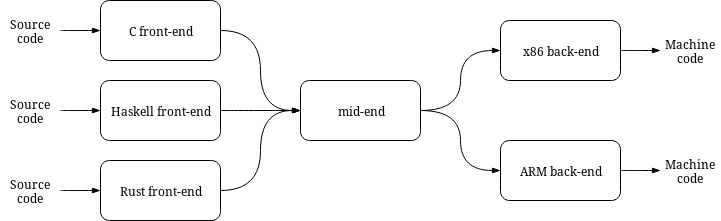
\includegraphics[width=12cm]{background/llvm/figures/three_phase_compiler}
	\caption{Three-phase compiler construction. The mid-end is somtimes called an \textit{optimizer}
	and the back-end a \textit{code generator}}
	\label{fig:three_phase_compiler}
\end{figure}

In the case of LLVM, the interface between the front-end and the mid-end is known as the
LLVM IR (\textit{Intermediate Representation}) and is a strongly typed, RISC-like virtual
instruction set that abstracts some details about the machine, such as function call
conventions and registers \cite[Section~11.3]{aosa-llvm}. To implement a programming language
one would then only have to implement a front-end, that is translate the source code to
LLVM IR. One could then pick and choose from the already existing LLVM optimizer passes
and LLVM back-end implementations to complete the compiler\cite[Section~11.5]{aosa-llvm}.

Only the back-end is of concern to this thesis, so it will focus exclusively on that.

\subsection{LLVM back-end}

A LLVM back-end, also known as a LLVM code generator, has a well defined input. The
LLVM IR\cite[Section~11.4.1]{aosa-llvm}. The output is often an object file, but a backend
can also act as an interpreter. For most of it's task, a LLVM backend uses what is called
the \textit{machine IR} to represent the code during the different stages.

% https://llvm.org/docs/WritingAnLLVMBackend.html
The LLVM back-end is responsible for three main tasks: intruction selection, instruction
scheduling and register allocation \cite{llvm-writing-backend, llvm-codegenerator-highlevel}.
They are performed mostly in isolation to each other, which simplifies the architecture
but introduces some interesting challenges "CITATION NEEDED".

The general behaviour of an LLVM back-end is that it transforms LLVM IR to machine code
for a specific target platform. Exactly what it produces depends on the target architecture
but it is common to generate assembly corresponding to the instruction set of the target
machine \cite[Section~11.5]{aosa-llvm}.

This paper does not cover instruction selection or other, smaller, back-end tasks such as
optimization, ABI implementation, exception handling etc \cite[at~1:47]{welcome-to-backend}.

\subsubsection{LLVM Machine Representation}

To represent machine specific IR LLVM uses what is called "Machine specific representation".
The machine specific representation consists of target agnostic, in-memory representations
of functions (MachineFuntion), basic blocks (MachineBasicBlock) and instructions
(MachinrInstr) \cite{llvm-mir-lang-ref, llvm-codegenerator-machinecode}.

The machine specific representation can be represented as the LLVM MIR (\textit{Machine
Intermediate Representation}), which is a human readable, YAML serialized format. It is
used to test code generation passes in LLVM. That is, we can stop the LLVM back-end
prematurely and view the current progress in the form of an LLVM MIR
\cite{llvm-mir-lang-ref}.

For example, the iterative factorial function written in C:

\lstinputlisting[language=C,tabsize=2,frame=single,breaklines=true,showstringspaces=false,
backgroundcolor= \color{lightgray}]
{background/llvm/examples/factorial.c}

gets translated to the following MIR when targeting the Hexagon V4 architecture and
terminating after instruction selection, right before register allocation and instruction
scheduling.

\lstinputlisting[tabsize=2,frame=single,breaklines=true,showstringspaces=false,
backgroundcolor= \color{lightgray}]
{background/llvm/examples/factorial.mir}

Courtesy of the Unison documentation for the code examples \cite{unison-docs-examples}.

What is interesting to note is that there is an infinite number of virtual registers available,
starting from \%0 and incrementing, as well as some abstract intructions, such as the PHI
function.

\subsubsection{Instruction Scheduling}
% https://llvm.org/docs/CodeGenerator.html#scheduling-and-formation
Instruction scheduling is the task of choosing how and in which order the selected instructions
will run. In the case of LLVM the scheduling phase is logically seperate from the selection
phase. There exists a wide variety of architecture and they all have different limitations
and constraints.

% https://llvm.org/devmtg/2016-09/slides/Absar-SchedulingInOrder.pdf - find better souce than this. Needs to be abou different archiectures
Perhaps the most intuitive kind of architecture is the in-order processor where all
instructions are executed sequentially and the schedule is staticically generated.

Alternatives to this architecture is and out-of-order processor where all instructions are
fetched and committed in-order, but executed out-of-order. In this case the instructions
are dynamically scheduled by the CPU. You can also have a VLIW (\textit{Very Long Instruction
Word}) processor where multiple instructions can be statically scheduled in parallel.

% http://infolab.stanford.edu/~ullman/dragon/w06/lectures/inst-sched.pdf - find better source for stuff like architecture, instruction scheduling goals and stuff.

As previously mentioned LLVM is a set of libraries, and thus no one way to schedule instructions
in LLVM exists. However, the key factors to take into account during instruction scheduling
is generally to make use of architecture specific features (such as VLIW), avoiding pipeline
stalls by rearranging instructions, reducing register pressure etc. When scheduling instructions
the main constraint is data-dependencies. Some instructions depends on the result of previous
instructions, and must thus be scheduled sequentially. In the cases where these dependencies
does not exists (or can be broken by e.g introducing new temporaries) the instructions
can be scheduled in a different order or in parallel (if the hardware allows it).

Instruction scheduling can be seen as a problem where the input is a list of resources
(e.g ALUs, FPUs, presence of VLIW) and a execution cycles for each instruction, and the
output is the instruction in the sequence they should be executed for optimal performance
(with regards to whatever factor you are optimizing for). In other words, maximize \textit{
	instruction level parallellism} "CITATION NEEDED". Of course this problem is very difficult.

\subsubsection{Register Allocation}
% https://llvm.org/pubs/2009-04-SCOPES-RegisterAllocationDeconstructed.pdf
% https://llvm.org/docs/CodeGenerator.html#register-allocator

This section needs

There are a few different problem concering register allocation, including (but not limied
to), coalescing, spilling move insertion and assigment \cite{alloc-deconstructed,
llvm-codegenerator-allocation}.

Coalescing is the attempt to eliminate move instructions that refers to identical locations,
i.e. remove unnecessary moves. When spilling a register you allocate the variable on the
stack to free up the register for another temporary ("spilling" the temporary to the stack)
and move insertion is used to split the lifetime of temporaries \cite{alloc-deconstructed}.

In general the task is modeled as a graph-coloring problem. The first step is then to
perform a \textit{liveliness analysis}, where you analyse the temporaries in the program
to determine which values has to co-exist (i.e. be placed in different registers). With
the liveliness analysis in hand a graph can be constructed where each node is a temporary,
edges represents that the two temporaries must be assigned to distinct registers and the
colors are registers. E.g for a machine with 64 registers you would use at most 64 colors
to color the graph. Assigning a temporary to a specific register (perhaps because of
calling conventions) would then be to "pre-color" the corresponding node. Coalescing in
this model would be to "merge" two nodes and spilling would be to remove a node. Spilling
is usually a consequence of not being able to find a coloring of the graph, thus
necessitating that a node be removed \cite{alloc-deconstructed}.

\subsubsection{Problems with LLVM Approach}
% http://i.stanford.edu/pub/cstr/reports/cs/tn/95/22/CS-TN-95-22.pdf
It is a common approach to treat instruction scheduling and register allocation as two
distinct steps in the back-end pipeline, and indeed so does LLVM. There are two approaches
to this, either you start with one or the other. Starting with instruction scheduling is,
nowadays, more common. Doing the register allocation first was mainly used in the early
days of compilers when machines didn't have as many registers \cite[\pno~3]{combining-alloc-sched}.

% citation needed
% maybe here: https://pdfs.semanticscholar.org/5246/7f742a206b075324ec17b9b7f9d539f52ec8.pdf
% it mentions that it needs to be merged which is good.
Seperating these steps in such a manner leads to some problems, and usually some instruction
scheduling is once again performed after the register allocation. If a register needs to be
spilled then the dependency graph which we based our schedule on is no longer valid. Re-doing
these steps is quite expensive though, as you would essentially throw out all previous
progress as soon as a register is spilled. Instead, modern compiler generate suboptimal
code. Not very modern.

% Mention the problem with offset and having to scavenge register
% https://youtu.be/objxlZg01D0?t=48m53s
More subtle, machine specific problems can also occur even after both instruction scheduling
and register allocation has happened. When setting up stack frames and resolving frame
indices one might find oneself in the situation of needing both additional instructions
\textit{and} more registers. This can occur because of the targets limited number of immediates,
for examples we might be doing something like this:

\lstinputlisting[tabsize=2,frame=single,breaklines=true,showstringspaces=false,
backgroundcolor= \color{lightgray}]
{background/llvm/examples/initial_inst.mir}

Where we attempt to store a value given a (symbolic) frame index. This frame index will be replaced by
the LLVM Prolog Epilog Inserter to a stack pointer and an offset. For example it might
generate something like this:

\lstinputlisting[tabsize=2,frame=single,breaklines=true,showstringspaces=false,
backgroundcolor= \color{lightgray}]
{background/llvm/examples/stack_offset.mir}

where it has replaced the frame index with an offset of 4104 from the stack pointer. However,
if the target cannot encode 4104 directly as an immediate we need another instruction to
calculate this offset, and another register to store the offset in, like so:

\lstinputlisting[tabsize=2,frame=single,breaklines=true,showstringspaces=false,
backgroundcolor= \color{lightgray}]
{background/llvm/examples/temporary_resources.mir}

Thus, we are in a situation where we need more instructions and more register after both
instruction scheduling and register allocation is already over. LLVM solves this with something
they call \textit{register scavenging}, which is not something that will be covered here
\cite[at~48:53]{welcome-to-backend}.

While this specific example might have needed to incorporate instruction selection into
the mix as well, it is nonetheless a difficulty.

% Citations for this. Unison, http://i.stanford.edu/pub/cstr/reports/cs/tn/95/22/CS-TN-95-22.pdf
% and find more.
Instruction selection, instruction scheduling and register allocation are all tasks that
depend on each other, but in order to make them managable by current solution they need
to be performed mostly in isolation to each other. Combining instruction scheduling and
register allocation is a popular subject of research.


% Contraint programming section
\section{Contraint Programming}

\subsection{Overview}

Constraint programming is a programming paradigm where problems are modeled as contraints
on variables. That is, a problem is solved by first identifying the variables, the domain
of each variable and the \textit{constraints} of the variables, i.e. the relation between them.
This is different from conventional programming paradigms because you are essentially
describing a solution to the problem, rather than an algorithm on how to achieve the solution.

Contraint programming is used to solve combinatorial problems in a relatively efficient
manner, which makes it an excellent approach to e.g. NP-problems. Constraint programming
is somtimes also called \textit{combinatorial optimization}, and implementations are then
% https://developers.google.com/optimization/
called \textit{combinatorial optimization software suite}. This is perhaps an ever better
name for the paradigm since it describes the usage (and limitations).

% https://en.wikipedia.org/wiki/Constraint_programming#Constraint_programming_libraries_for_imperative_programming_languages
This paradigm is not limited to certain languages but are usually implemented as libraries
that implement a constraint solver. There are also a few languages that support constraint
programming natively, such as Curry.
% http://www-ps.informatik.uni-kiel.de/currywiki/_media/documentation/report.pdf
% http://www-ps.informatik.uni-kiel.de/currywiki/documentation/features
In both cases the user specifies the variables and
the constraints and the constaint solver propagates the given constraints and reduces each
variable's domain until there is only one option left, and the problem is solved.

\subsection{Modeling a Problem}

To illustrate how to model and solve problems with constraint programming consider the
following example.

We are presented with the problem of solving the equation $SEND + MOST = MONEY$, where
each letter is to be subsituted with a digit, $S$ and $M$ cannot be 0, and all digits must
be pairwise distinct. We can easily determine that this is indeed a combinatorial problem
and that, presumably, there exists multiple solutions. The naive method of solving this
problem would be with an exhaustive search. However, this would try a lot of combinations
that can analytically be determined to \textit{not} be part of a solution. To do better we
will employ constraint programming and model the problem in 4 steps:

\begin{enumerate}
	\item Identifying variables and corresponding domains
	\item Determining constraints
	\item Choosing a search heuristic
	\item Optimizing
\end{enumerate}

\subsubsection{Identifying Variables and Corresponding Domains}

The first step of modeling is to determine the variables of the problem, and what their
possible values are. The set of possible values is refered to as the variable's \textit{
domain}. Choosing the variables of a problem is not always easy and the implications
of the choice may not be apparent until later steps. E.g. for certain problems the intuitive
variable selection might make searching too inefficient to ever terminate. In our case
choosing variables is very straightforward. We have one variable for each letter. Since
each letter is the be replaced with a digit the domain of each variable is 0 through 9.

\vspace{0.5cm}
\noindent
$S \in \{0, 1, 2, 3, 4, 5, 6, 7, 8, 9\}$ \\
$E \in \{0, 1, 2, 3, 4, 5, 6, 7, 8, 9\}$ \\
$N \in \{0, 1, 2, 3, 4, 5, 6, 7, 8, 9\}$ \\
$D \in \{0, 1, 2, 3, 4, 5, 6, 7, 8, 9\}$ \\
$M \in \{0, 1, 2, 3, 4, 5, 6, 7, 8, 9\}$ \\
$O \in \{0, 1, 2, 3, 4, 5, 6, 7, 8, 9\}$ \\
$T \in \{0, 1, 2, 3, 4, 5, 6, 7, 8, 9\}$ \\
$Y \in \{0, 1, 2, 3, 4, 5, 6, 7, 8, 9\}$

Henceforth two integers seperated by two dots will indicate a range of all integers between
and including the two specified.

\subsubsection{Determining Constraints}

The constraints of our model is used to describe the relationship between variables in a
solution. For example how does $S$ and $E$ interact when part of a solution? Given the
problem describtion one constraint is that each digit is only used once, i.e. our variables
are pairwise distinct. If $S$ is assigned 1, no other letter can be assigned 1. In addition,
both $S$ and $M$ are nonzero, so we post one constraint for each that excludes 0 from their
domain.

To enforce the equation in the problem description we post the constraint: \\

\begin{tabular}{cccccc}
	& & $1000 * S$ & $100 * E$ & $10 * N$ & $D$ \\
	+ &	& $1000 * M$ & $100 * O$ & $10 * S$ & $T$ \\
	\hline
	& $10000 * M$ & $1000 * O$ & $100 * N$ & $10 * E$ & $Y$
\end{tabular}

If all of these constraints are true for a certain mapping of letters to digits, that
mapping is considered a solution to the problem.

\subsubsection{Propagating}

To find a solution we start by \textit{propagating} these constraint. Propagating a constraint
means that for every constraint we check which values in a variable's domain are incompatible
with the constraint. I.e. we exclude values that can never be part of a solution. In this
case, we have one constraint for $S$ and one constraint for $M$ that say that they must
be nonzero. We can thus remove the 0 from their domains. We systematically work through
all constraints and keep pruning values from domains.

% TODO The variables and their domains after propagation for the example
If we propagate the given constraints on the initial domains of our variables we are left
with the following state:

\vspace{0.5cm}
\noindent
$S \in \{9\}$ \\
$E \in \{2..7\}$ \\
$N \in \{3..8\}$ \\
$D \in \{2..8\}$ \\
$M \in \{1\}$ \\
$O \in \{0\}$ \\
$T \in \{2..8\}$ \\
$Y \in \{2..8\}$

Notably, we have already determined that $S$ has to be 9, which excludes it from all other
domains. In a similar manner we have assigned $M=1$ and $O=0$ and removed 1 and 0 from all
other domains, this in turn has led to the exclusion of 2 from the domain of $N$. In other
words, the equation will look something like $9END + 109T = 10NEY$

When no more domains can be pruned we have one of three situations. One or more domain(s)
could be empty, proving that no solution exists. All domains could be of size 1, indicating
that there exists only one possible value for every variable, and thus we have found a
solution. And last but not least, one or more variables have multiple values in their
domain. If we reach any of the former situations, either a solution is found or we have proven
that a solution does not exist. In the latter situation we have multiple possbile values,
and we must explore these combinations. We do that by \textit{branching}.

\subsubsection{Searching}

To explore the different combinations of variable to value mappings we construct a \textit{
search tree}. Each node of the search tree constists of every variable and their respective
domain after propagation. The root node would then be the all variables and their domains
after initial propagation (as in the previous section). From each node we create two or
more branches, where each branch represents a subset of a domain for a particular variable.
For example, we could create one branch were $E \in \{2..4\}$ and one branch where $E \in 
\{5..7\}$. It is important that the branches completely covers the original
domain, so that all possible values are explored.

We will then follow one of the branches, propagate constraints given the reduced domain
of the branching variable and once again reach one of the three previously mentioned
situations, only in this case if we have reached the first situation (failure) we can go
back and go down the other branch. This process is applied recuresively until a solution
is found or all combinations have been exhausted.

\subsubsection{Choosing a branching heuristic}

Determining on which variable to branch, how many branches to create and which values to
include or exclude for every branch is very much dependent on the problem being modeled.
In this case something simple is sufficient and we can say that when a dead-end is reached
we pick the variable with the smallest domain and create one branch where that variable
is mapped to the smallest value in that domain, and one branch where the smallest value
is excluded from the domain.

\begin{figure}[h]
	\centering
	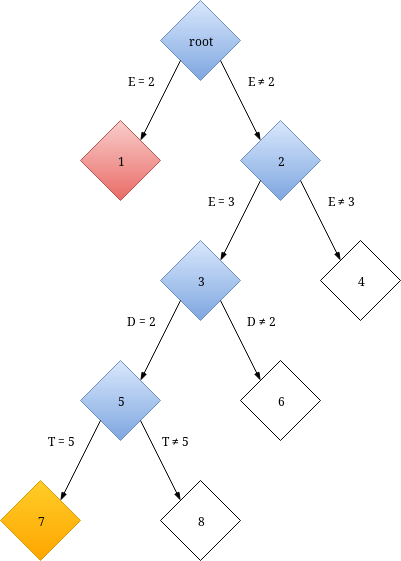
\includegraphics[width=8cm]{background/constraint-programming/figures/constraint_first_solution}
	\caption{Search tree of first solution to SEND+MOST=MONEY problem.
	White nodes are unvisited, blue nodes are propagated, red nodes are failed and orange nodes are solutions.}
	\label{fig:first_solution}
\end{figure}

\begin{table}
	\centering
	\begin{tabular}{c|c|c|c|c|c|c|c|c}
		Node & S & E & N & D & M & O & T & Y \\
		\hline
		root & 9 & {2..7} & {3..8} & {2..8} & 1 & 0 & {2..8} & {2..8} \\
		2 & 9 & {3..7} & {4..8} & {2..8} & 1 & 0 & {2..8} & {2..8} \\
		3 & 9 & 3 & 4 & {2, 5, 6} & 1 & 0 & {2, 5, 6} & {5..8} \\
		5 & 9 & 3 & 4 & 2 & 1 & 0 & {5, 6} & {7, 8} \\
		7 & 9 & 3 & 4 & 2 & 1 & 0 & 5 & 7 \\
	\end{tabular}
	\caption{Each variable's domain in the nodes (after propagation) explored to reach the first solution}
	\label{tab:first_solution_states}
\end{table}

Figure \ref{fig:first_solution} shows all branching made to reach the first solution given
our branching heuristic. Table \ref{tab:first_solution_states} show the domains of each
variable at a given node (after propagation). Node 7 represents a solution to the problem,
namely $9342+1095=10437$.

\subsubsection{Optimizing}
\label{sec:optimizing}

As previously mentioned constraint programming is sometimes called combinatorial optimization.
Optimizing the solution is done during the search. When we find a solution by searching,
instead of terminating the program and returning the found solution we apply an additional
constraint that says that from now on, a combination will only be considered a solution
if it is \textit{better} than the current solution. If we find another solution, we can
set the bar at that solution instead. This process is called \textit{branch and bound}.

For a combinatioral problem we expect mutliple solutions, and by always requiring the
next solution to be better than the last we will eventually, given enough time, reach
the \textit{optimal} solution. That is if we apply a branch and bound strategy and allow
it to run until termination, we have both found the optimal solution and proved that it is
the optimal solution. For large problems however, this might take an unreasonable amount
of time and it is better to terminate early.

The first step of finding the optimal solution is indentify what constintutes as \textit{
	better}. In our case we want as much money as possible. One solution is better than
another one if the mapping of $MONEY$ yields a larger integer. Table \ref{tab:two_solutions}
shows two distinct solutions, one better than the other.
% Provide example with two solutions

\begin{table}
	\centering
	\begin{tabular}{c|c|c|c|c|c|c|c|c}
		S & E & N & D & M & O & T & Y & MONEY \\
		\hline
		9 & 3 & 4 & 2 & 1 & 0 & 5 & 7 & 10437 \\
		9 & 3 & 4 & 2 & 1 & 0 & 6 & 8 & 10438 \\
	\end{tabular}
	\caption{Two solution to the problem, one better than the other.}
	\label{tab:two_solutions}
\end{table}

For every solution we find, we require subsequent solution to map $MONEY$ to a larger
integer. The optimal solution is the largest integer for $MONEY$ we can find while still
conforming to all constraints. If we keep searching and keep requiring that the next solution
is better than the last we will eventually conclude that the optimal solution is the one
presented in table \ref{tab:optimal_solution}.

\begin{table}
	\centering
	\begin{tabular}{c|c|c|c|c|c|c|c|c}
		S & E & N & D & M & O & T & Y & MONEY \\
		\hline
		9 & 7 & 8 & 2 & 1 & 0 & 4 & 6 & 10876 \\
	\end{tabular}
	\caption{The optimal solution.}
	\label{tab:optimal_solution}
\end{table}

% Source code in appendix TODO: figure out which appendix
The source code, written with Gecode, for the problem can be found in appendix
\ref{appendix:constraint_programming}.

\subsection{Summary}
The most important part of constraint programming is that you are describing how a
solution to a problem looks, not how to calculate that solution. This in turn makes it
good for combinatorial problems, where you can quickly exclude certain combinations thanks
to early detection of illegal values. By then creating a \textit{search tree}, where each
node represents a particular state of variables and their respective domains and each
branch represents limiting a variable's domain to a subset of the previous state. When
searching for solutions one can require that the next candidate is only considered a solution
if it is in some way \textit{better} than the previous solution, thus eventually yielding
the optimal solution.


% Unison
\section{Unison}
\label{sec:unison}

Unison is an open-source\footnote{\url{https://github.com/unison-code/unison}},
potentially optimal tool that performs integrated register allocation and instruction
scheduling using constraint programming. It can be used as an alternative or complement to
the algorithms currently in place by compilers such as GCC and LLVM. In particular there
already exists a driver for LLVM which accept input in the form of LLVM MIR \cite{unison-docs}.

\subsection{Constraint Programming}

Constraint programming is a programming paradigm for solving combinatorial problems.
By declaring all variables possible values and their \textit{constraints}, the relationship
between them when part of a solution, a \textit{constraint solver} can search the solution
space and find an assignment of variables to values that is consistent with the constraints.
A constraint solver effectively explores different possible combinations systematically,
by a potentially incomplete local inference (also known as \textit{constraint propagation})
or more commonly a combination of the two \cite{handbook-constraint-programming}.

Currently the only constraint solver supported by Unison is Gecode\footnote{\url{www.gecode.org}}
\cite{unison-docs}, which is a constraint solver that interleaves system search algorithms
search with constraint propagation\cite{MPG}.

When propagating constraints the Gecode solver searches all variable's domains and removes
variables that in conflict with the constraints\cite[Section~23.1]{MPG}. For example,
given two variables (and their corresponding domains) $x \in {0,1,2}$ and $y \in {0,1,2}$
and the constraint $x > y$ constraint propagation can determine that $x \in {1, 2}$ and
$y \in {0, 1}$ are the only combinations consistent with the constraint.

When constraint propagation is finished there are three possible states:

\begin{enumerate}
	\item One or more domains could be empty, proving that no solution exists.
	\item	All domains could be of size 1, indicating that there exists only one possible
		value for every variable, and thus we have found a solution.
	\item One or more variables have multiple values in their domain.
\end{enumerate}

For situation (1) and (2), either a solution is found or we have proven that a solution
does not exist (within the local search space).

In the latter situation (3) the Gecode constraint solver splits a variable's domain into
two or more subsets, creating a \textit{search tree} where each \textit{branch} represents
reducing the variable's domain to a particular subset \cite[Section~8]{MPG}. By commiting
to a branch the constraint solver can once again perform constraint propagation and repeat
the process. However, if \textit{branching} has taken place and the solver reaches
situation (1) it can go back up the tree and explore a different branch. If situation (2)
is reached it can still backtrack but with the added option of adding more constraints
based on the newly found solution. Constraining based on previously found solutions in the
search tree is done with the \textit{branch-and-bound} search engine\cite[Section~9]{MPG}
in Gecode.

\textit{Branch and bound} is an efficient strategy to find the optimal solution to a
combinatorial problem which in essence constitutes comparing potential solutions to the
currently best found solution, choosing the better of the two\cite{BaB}. We will adopt a
similar strategy, but instead of constraining solutions to be better we will require them
to be \textit{different}. In addition, no solutions will be discarded.

\subsection{Unison}


Unison models the problems of register allocation and instruction scheduling as a single
constraint-satisfaction problem and solves them simultaneously \cite{unison-docs,reg-alloc-inst-sched-uni}.

Unison's key properties are that it introduces \textit{optional copies} and
\textit{alternative temporaries} \cite{reg-alloc-inst-sched-uni}. This allows Unison to
support different register allocation decision and perform otherwise unreachable optimizations
\cite{reg-alloc-inst-sched-uni, comb-spill}.



% Method
\chapter{Exploring the Unison Diversity Space}

\section{What do we want to do?}


\section{How much variation do we tolerate?}

Does all binaries have to be within a (e.g) 5-cycle cost of each other? Can we just spit something
out every X seconds and assume it's different enough? Can we choose the variation depending
on how many binaries the user wants? 


% Bibliography
\printbibliography[heading=bibintoc] % Print the bibliography (and make it appear in the table of contents)

% Appendices
\appendix

% Appendix A
\chapter{Unnecessary Appended Material}

\chapter{SEND+MOST=MONEY Source Code}
\label{appendix:constraint_programming}
\lstinputlisting[language=C++,tabsize=2,frame=single,breaklines=true,showstringspaces=false]
	{background/examples/send_most_money.cpp}

\end{document}
